\documentclass[UTF8]{ctexart}
\usepackage{setspace}
\usepackage[letterpaper,top=2cm,bottom=2cm,left=3cm,right=3cm,marginparwidth=1.75cm]{geometry}
\usepackage{listings}
\usepackage{xcolor}      %代码着色宏包
\usepackage{amsmath}
\usepackage{mathabx}\usepackage{amssymb}
\usepackage{tikz}
\usepackage{verbatim}
\usepackage[mathscr]{eucal}
\usepackage{graphicx}
\usepackage{caption}
\usepackage{subfigure}
\CTEXsetup[format={\Large\bfseries}]{section}

\title{数学软件作业2-王锦宸}
\author{数学与应用数学2002 王锦宸}
\date{July 2023}

\begin{document}

\maketitle

\section*{12.2 不可压缩的纳维-斯托克斯方程}
不可压缩流体的二维流场完全由速度矢量$q=(u(x,y),v(x,y))\in \mathbb{R}^2$和压力$p(x,y)\in \mathbb{R}$描述。这些函数是下列守恒定律的解(例如,见Hirsch, 1988):
\begin{itemize}
    \item 质量守恒:
\end{itemize}
\begin{equation}
    \operatorname{div}(q)=0\label{12.1}
\end{equation}

\indent 或者,用发散\footnote{我们回顾一下二维场的微分算子发散、梯度和拉普拉斯的定义:如果 $v=\left(v_x, v_y\right): \mathbb{R}^2 \mapsto \mathbb{R}^2$ and $\varphi: \mathbb{R}^2 \mapsto \mathbb{R}$, 那么$$
\operatorname{div}(v)=\frac{\partial v_x}{\partial x}+\frac{\partial v_y}{\partial y}, \quad \mathcal{G} \varphi=\left(\frac{\partial \varphi}{\partial x}, \frac{\partial \varphi}{\partial y}\right), \quad \Delta \varphi=\operatorname{div}(\mathcal{G} \varphi)=\frac{\partial^2 \varphi}{\partial x^2}+\frac{\partial^2 \varphi}{\partial y^2},
$$.
且 $\Delta v=\left(\Delta v_x, \Delta v_y\right)$.}算子的明确形式来写、
\begin{equation}
    \frac{\partial u}{\partial x}+\frac{\partial v}{\partial y}=0\label{12.2}
\end{equation}

\begin{itemize}
    \item 动量守恒方程的闭形式\footnote{我们用$\otimes$表示张量乘积.}
\end{itemize}
\begin{equation}
    \frac{\partial q}{\partial t}+\operatorname{div}(q \otimes q)=-\mathcal{G} p+\frac{1}{R e} \Delta q
    \label{12.3}
\end{equation}
\indent 或,使用外显形式
\begin{equation}
    \left\{\begin{array}{l}
\frac{\partial u}{\partial t}+\frac{\partial u^2}{\partial x}+\frac{\partial u v}{\partial y}=-\frac{\partial p}{\partial x}+\frac{1}{R e}\left(\frac{\partial^2 u}{\partial x^2}+\frac{\partial^2 u}{\partial y^2}\right) \\
\frac{\partial v}{\partial t}+\frac{\partial u v}{\partial x}+\frac{\partial v^2}{\partial y}=-\frac{\partial p}{\partial y}+\frac{1}{R e}\left(\frac{\partial^2 v}{\partial x^2}+\frac{\partial^2 v}{\partial y^2}\right)
\end{array}\right.
\label{12.4}
\end{equation}





\indent 前面的方程以无量纲形式写出,使用以下比例的变量:
\begin{equation}
    x=\frac{x^*}{L}, \quad y=\frac{y^*}{L}, \quad u=\frac{u^*}{V_0}, \quad v=\frac{v^*}{V_0}, \quad t=\frac{t^*}{L / V_0}, \quad p=\frac{p^*}{\rho_0 V_0^2},
    \label{12.5}
\end{equation}

\indent 其中上标(*)表示以物理单位测量的变量。常数$L, V_0$分别是模拟流动的特征的参考长度和速度。无量纲数$R e$被称为雷诺数,用于量化流动中惯性(或对流)项和粘性(或扩散)${ }^3$项的相对重要性:
\begin{equation}
    R e=\frac{V_0 L}{\nu}
    \label{12.6}
\end{equation}

其中$\nu$是流动的运动黏度。
综上所述,本项目中要数值求解的Navier-Stokes PDEs系统由\ref{12.2}和\ref{12.4}定义;初始条件(在$t=0$时)和边界条件将在以下章节中讨论。

\section*{12.4 计算域、交错网格和边界条件}
通过考虑一个矩形域$L_x\times L_y$(见图1),并在各处设置周期性边界条件,可以大大简化纳维-斯托克斯方程的数值求解。速度$q(x, y)$和压力$p(x, y)$场的周期性在数学上表示为
\begin{equation}
    \begin{array}{lll}
    q(0, y)=q\left(L_x, y\right), & p(0, y)=p\left(L_x, y\right), & \forall y \in\left[0, L_y\right]\\
    q(x, 0)=q\left(x, L_y\right), & p(x, 0)=p\left(x, L_y\right), & \forall x \in\left[0, L_x\right]
    \end{array}
    \label{12.7}
\end{equation}

\indent 计算解决方案的点是按照一个矩形的、统一的2D的网格分布在域中。由于在我们的方法中不是所有的变量都在同一个网格中,我们首先定义一个主网格(图12.1),分别沿$x$取$n_x$计算点和沿$y$取$n_y$点来生成:

\begin{equation}
    \begin{aligned}
    & x_c(i)=(i-1) \delta x, \quad \delta x=\frac{L_x}{n_x-1}, \quad i=1, \ldots, n_x, \\
    & y_c(j)=(j-1) \delta y, \quad \delta y=\frac{L_i}{n_y-1}, \quad j=1, \ldots, n_y
    \end{aligned}
    \label{12.8}
\end{equation}

\begin{figure}[h]
\centering  %居中
\subfigure[]{   %第一张子图
\begin{minipage}{7cm}
\centering    %子图居中
\tikzset{every picture/.style={line width=0.75pt}} %set default line width to 0.75pt        

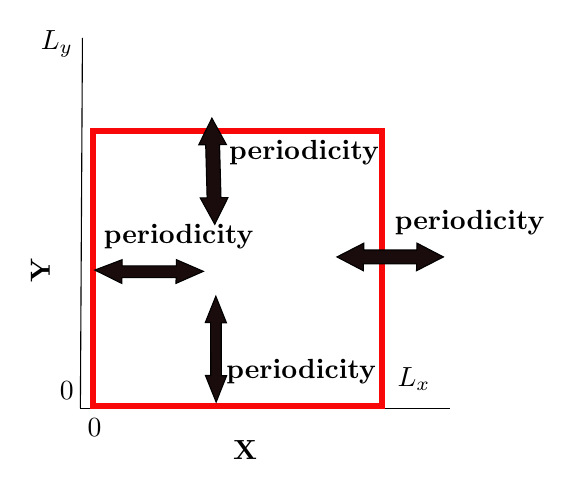
\begin{tikzpicture}[x=0.75pt,y=0.75pt,yscale=-1,xscale=1]
%uncomment if require: \path (0,300); %set diagram left start at 0, and has height of 300

%Straight Lines [id:da8860806918844237] 
\draw    (262.71,233.72) -- (440.78,233.72) ;
%Straight Lines [id:da2482364951571545] 
\draw    (263.71,55.29) -- (262.71,233.72) ;
%Shape: Rectangle [id:dp8363663747990173] 
\draw  [color={rgb, 255:red, 248; green, 8; blue, 8 }  ,draw opacity=1 ][line width=2.25]  (268.85,100) -- (407.9,100) -- (407.9,232.7) -- (268.85,232.7) -- cycle ;
%Left Right Arrow [id:dp14914306169840552] 
\draw  [fill={rgb, 255:red, 26; green, 12; blue, 12 }  ,fill opacity=1 ] (269.68,167.15) -- (282.85,162.15) -- (282.8,165.15) -- (308.93,165.15) -- (308.98,162.15) -- (321.95,167.76) -- (308.78,173.56) -- (308.83,170.76) -- (282.7,170.76) -- (282.65,173.56) -- cycle ;
%Left Right Arrow [id:dp5889856701294844] 
\draw  [fill={rgb, 255:red, 26; green, 12; blue, 12 }  ,fill opacity=1 ] (326.07,93.98) -- (333.09,106.73) -- (329.76,106.73) -- (330.45,132.27) -- (333.79,132.27) -- (327.46,145.07) -- (320.45,132.36) -- (323.78,132.36) -- (323.09,106.79) -- (319.75,106.79) -- cycle ;
%Left Right Arrow [id:dp10007282723892508] 
\draw  [fill={rgb, 255:red, 26; green, 12; blue, 12 }  ,fill opacity=1 ] (327.97,179.76) -- (333.11,192.58) -- (330.56,192.58) -- (330.63,218.07) -- (333.18,218.07) -- (328.12,230.74) -- (322.98,217.96) -- (325.53,217.96) -- (325.46,192.43) -- (322.91,192.43) -- cycle ;
%Left Right Arrow [id:dp7200416632481255] 
\draw  [fill={rgb, 255:red, 26; green, 12; blue, 12 }  ,fill opacity=1 ] (386.33,160.82) -- (399.27,154.19) -- (399.21,157.5) -- (424.85,157.5) -- (424.91,154.19) -- (437.61,160.82) -- (424.67,167.45) -- (424.73,164.13) -- (399.09,164.13) -- (399.03,167.45) -- cycle ;

% Text Node
\draw (242.38,50.63) node [anchor=north west][inner sep=0.75pt]    {$L_{y}$};
% Text Node
\draw (414.3,212.74) node [anchor=north west][inner sep=0.75pt]    {$L_{x}$};
% Text Node
\draw (272.74,144.01) node [anchor=north west][inner sep=0.75pt]   [align=left] {\textbf{periodicity}};
% Text Node
\draw (333.12,103.22) node [anchor=north west][inner sep=0.75pt]   [align=left] {\textbf{periodicity}};
% Text Node
\draw (412.94,136.87) node [anchor=north west][inner sep=0.75pt]   [align=left] {\textbf{periodicity}};
% Text Node
\draw (331.75,208.67) node [anchor=north west][inner sep=0.75pt]   [align=left] {\textbf{periodicity}};
% Text Node
\draw (251.52,219.86) node [anchor=north west][inner sep=0.75pt]    {$0$};
% Text Node
\draw (264.91,237.34) node [anchor=north west][inner sep=0.75pt]    {$0$};
% Text Node
\draw (237.59,174.59) node [anchor=north west][inner sep=0.75pt]  [rotate=-270] [align=left] {\textbf{Y}};
\draw (335,248) node [anchor=north west][inner sep=0.75pt]  [rotate=0] [align=left] {\textbf{X}};

\end{tikzpicture}  %以pic.jpg的0.5倍大小输出
\end{minipage}
}
\subfigure[]{ %第二张子图
\begin{minipage}{7cm}
\centering    %子图居中
\tikzset{every picture/.style={line width=0.75pt}} %set default line width to 0.75pt        

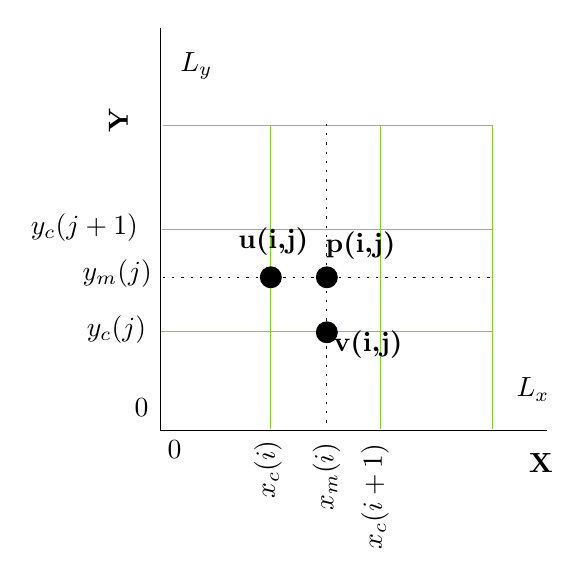
\begin{tikzpicture}[x=0.75pt,y=0.75pt,yscale=-1,xscale=1]
%uncomment if require: \path (0,300); %set diagram left start at 0, and has height of 300

%Straight Lines [id:da11452555740391301] 
\draw    (226.88,230.15) -- (412.88,230.15) ;
%Straight Lines [id:da887351631569798] 
\draw    (226.88,36.15) -- (226.88,230.15) ;
%Straight Lines [id:da038658005061680045] 
\draw [color={rgb, 255:red, 126; green, 211; blue, 33 }  ,draw opacity=1 ]   (226.88,182.15) -- (386.88,182.15) ;
%Straight Lines [id:da7430443309836143] 
\draw [color={rgb, 255:red, 126; green, 211; blue, 33 }  ,draw opacity=1 ]   (227.38,133.15) -- (386.88,133.15) ;
%Straight Lines [id:da3754320940133724] 
\draw [color={rgb, 255:red, 126; green, 211; blue, 33 }  ,draw opacity=1 ]   (227.88,83.15) -- (386.88,83.15) ;
%Straight Lines [id:da6619177081180496] 
\draw [color={rgb, 255:red, 126; green, 211; blue, 33 }  ,draw opacity=1 ]   (279.88,83.15) -- (279.88,229.15) ;
%Straight Lines [id:da9440624237128155] 
\draw [color={rgb, 255:red, 126; green, 211; blue, 33 }  ,draw opacity=1 ]   (332.88,83.15) -- (332.88,229.15) ;
%Straight Lines [id:da052561514407487575] 
\draw [color={rgb, 255:red, 126; green, 211; blue, 33 }  ,draw opacity=1 ]   (386.88,83.15) -- (386.88,229.15) ;
%Straight Lines [id:da7981659736721409] 
\draw  [dash pattern={on 0.84pt off 2.51pt}]  (306.88,82.15) -- (306.88,230.15) ;
%Straight Lines [id:da19820007165593956] 
\draw [color={rgb, 255:red, 0; green, 0; blue, 0 }  ,draw opacity=1 ] [dash pattern={on 0.84pt off 2.51pt}]  (227.88,156.15) -- (306.88,156.15) -- (386.88,156.15) ;
%Shape: Circle [id:dp7090163098190359] 
\draw  [fill={rgb, 255:red, 0; green, 0; blue, 0 }  ,fill opacity=1 ] (301.88,156.15) .. controls (301.88,153.39) and (304.11,151.15) .. (306.88,151.15) .. controls (309.64,151.15) and (311.88,153.39) .. (311.88,156.15) .. controls (311.88,158.91) and (309.64,161.15) .. (306.88,161.15) .. controls (304.11,161.15) and (301.88,158.91) .. (301.88,156.15) -- cycle ;
%Shape: Circle [id:dp494169418492836] 
\draw  [fill={rgb, 255:red, 0; green, 0; blue, 0 }  ,fill opacity=1 ] (301.88,182.65) .. controls (301.88,179.89) and (304.11,177.65) .. (306.88,177.65) .. controls (309.64,177.65) and (311.88,179.89) .. (311.88,182.65) .. controls (311.88,185.41) and (309.64,187.65) .. (306.88,187.65) .. controls (304.11,187.65) and (301.88,185.41) .. (301.88,182.65) -- cycle ;
%Shape: Circle [id:dp6555607910805403] 
\draw  [fill={rgb, 255:red, 0; green, 0; blue, 0 }  ,fill opacity=1 ] (274.88,156.15) .. controls (274.88,153.39) and (277.11,151.15) .. (279.88,151.15) .. controls (282.64,151.15) and (284.88,153.39) .. (284.88,156.15) .. controls (284.88,158.91) and (282.64,161.15) .. (279.88,161.15) .. controls (277.11,161.15) and (274.88,158.91) .. (274.88,156.15) -- cycle ;

% Text Node
\draw (305,133) node [anchor=north west][inner sep=0.75pt]   [align=left] {\textbf{p(i,j)}};
% Text Node
\draw (263,131) node [anchor=north west][inner sep=0.75pt]   [align=left] {\textbf{u(i,j)}};
% Text Node
\draw (308.88,180.65) node [anchor=north west][inner sep=0.75pt]   [align=left] {\textbf{v(i,j)}};
% Text Node
\draw (163,124.4) node [anchor=north west][inner sep=0.75pt]    {$y_{c}( j+1)$};
% Text Node
\draw (190,173.4) node [anchor=north west][inner sep=0.75pt]    {$y_{c}( j)$};
% Text Node
\draw (188,146.4) node [anchor=north west][inner sep=0.75pt]    {$y_{m}( j)$};
% Text Node
\draw (213,213.4) node [anchor=north west][inner sep=0.75pt]    {$0$};
% Text Node
\draw (228.88,233.55) node [anchor=north west][inner sep=0.75pt]    {$0$};
% Text Node
\draw (270.54,264.08) node [anchor=north west][inner sep=0.75pt]  [rotate=-270]  {$x_{c}( i)$};
% Text Node
\draw (298.71,269.87) node [anchor=north west][inner sep=0.75pt]  [rotate=-270]  {$x_{m}( i)$};
% Text Node
\draw (322.1,288.56) node [anchor=north west][inner sep=0.75pt]  [rotate=-270]  {$x_{c}( i+1)$};
% Text Node
\draw (200.65,87.71) node [anchor=north west][inner sep=0.75pt]  [rotate=-270] [align=left] {\textbf{Y}};
% Text Node
\draw (402.98,240.02) node [anchor=north west][inner sep=0.75pt]  [rotate=0] [align=left] {\textbf{X}};
% Text Node
\draw (235,46.4) node [anchor=north west][inner sep=0.75pt]    {$L_{y}$};
% Text Node
\draw (397,203.4) node [anchor=north west][inner sep=0.75pt]    {$L_{x}$};


\end{tikzpicture}
%以pic.jpg的0.5倍大小输出
\end{minipage}
}
\caption{计算域、交错网格和边界条件}    %大图名称
\label{fig:1}    %图片引用标记
\end{figure}
%此处插入图片,下面的是图片的名字
%图12.1. 
\indent 二级网格是由一级网格单元的中心定义的:
\begin{equation}
    \begin{array}{ll}
        x_m(i)=(i-1 / 2) \delta x, & i=1, \ldots, n_{x m}, \\
        y_m(j)=(j-1 / 2) \delta y, & j=1, \ldots, n_{\mathrm{g} m},
    \end{array}
    \label{12.9}
\end{equation}

\indent 其中我们使用了$n_{x m}=n_x-1, n_{y m}=n_y-1$的简记符号。在定义为矩形$[x_c(i), x_c(i+1)] \times [y_c(j), y_c(j+1)]$ 的计算单元内,未知变量 $u, v, p$将被计算为不同空间位置的解决方案的近似值:
\begin{itemize}
    \item $u(\dot{x}, j) \approx u\left(x_c(i), y_m(j)\right)$ (计算单元的西面)
    \item $v(i, j)\approx v\left(x_m(i), y_c(j)\right)$ (计算单元的南面)
    \item $p(i, j)\approx p\left(x_m(i), \psi_m(j)\right)$ (计算单元的中心)
\end{itemize}
\par 这种变量的交错排列具有压力和速度之间强烈耦合的优点。它还有助于(见本章末尾的参考文献\cite{thebook})避免同位排列(所有变量都在同一网格点上计算)所遇到的一些稳定性和收敛性问题。

\bibliographystyle{plain}
\bibliography{references}

\end{document}
